
\documentclass[a4paper,11pt]{article}

%\usepackage{marvosym}
\usepackage{amsmath}
\usepackage{amssymb}
\usepackage{verbatim}
\usepackage{graphicx}
\usepackage{psfrag}
\usepackage{listings}
\usepackage{booktabs}
\usepackage{caption}
\usepackage{subcaption}

% MARGIN SETTINGS
\setlength{\voffset}{-1.1in}
\setlength{\textheight}{740pt}
%\setlength{\topmargin}{-0.5in}
\setlength{\textwidth}{6.2in}
\setlength{\oddsidemargin}{0.1in}
\setlength{\evensidemargin}{0in}
\setlength{\footskip}{20pt}

\author{Will Booker}
\title{Compressible Acoustic Waves}

\begin{document}

\maketitle

\section{Preliminaries}


A Hamiltonian formulation is a system with either an finite or infinite number of degrees of freedom with a specified structure. The system's dynamics are then described in phase-space using two geometric objects: a total energy functional,  the Hamiltonian $\mathcal{H}$, and a skew symmetric Poisson bracket $\{ , \}$.
As systems of fluid dynamics are continuous in space, we will be considering infinite dimensional dynamical systems. 



 We now consider the general state of a functional $\mathcal{F}$ for  the system in consideration, the functional's time evolution is now described by the following equation,

\begin{equation}
 \frac{ d \mathcal{F}}{dt} =\{\mathcal{F},\mathcal{H}\} .
\end{equation}
The Poisson bracket has to satisfy the following conditions :

\begin{itemize}
\item skew-symmetry: $\{\mathcal{F},\mathcal{H}\}$ = $-\{\mathcal{H},\mathcal{F}\}$,
\item linearity: $\{\alpha \mathcal{F} + \beta \mathcal{G},\mathcal{H}\}$ = $\alpha \{\mathcal{F},\mathcal{H}\}$ + $\beta\{\mathcal{G},\mathcal{H}\}$,
\item Jacobi identity: $ \{\mathcal{F},\{\mathcal{G},\mathcal{H}\}\}$ + $ \{\mathcal{G},\{\mathcal{H},\mathcal{F}\}\}$ + $ \{\mathcal{H},\{\mathcal{F},\mathcal{G}\}\}$ = 0,
\item Leibniz identity:   $\{\mathcal{F}\mathcal{G},\mathcal{H}\}$ = $\mathcal{F}\{\mathcal{G},\mathcal{H}\}$ + $\{\mathcal{F},\mathcal{H}\}\mathcal{G}$,
\end{itemize}
where $\alpha$, $\beta$ are constants, and $\mathcal{F}$, $\mathcal{G}$, $\mathcal{H}$ are arbitrary functionals. \\
We  note that the skew-symmetry condition automatically yields energy conservation for the system,
\[\frac{d \mathcal{H}}{dt} = \{\mathcal{H},\mathcal{H}\}= -\{\mathcal{H},\mathcal{H}\} = 0.\]
We first  need to define a variational derivative, 
\begin{equation}\label{eqns:var_deriv}
\delta \mathcal{H} = \lim_{\epsilon \rightarrow 0}\frac{ \mathcal{H}( u+ \epsilon\delta u)-  \mathcal{H}(u)}{\epsilon}= \bigg ( \frac{\delta  \mathcal{H}}{\delta u}, \delta u \bigg)+  \mathcal{O}(\delta u^2),
\end{equation}
where $(\cdot,\cdot)$ is the inner product for the function space $\{ u\}$.



\section{Continuum Description}

In this report we will consider in a compressible fluid in a one-dimensional domain $\Omega$ . We will assume that viscous effects and temperature effects do not influence the motion of the fluid. We assume that the resting density, $\rho_0$ and acoustic speed of sound $c^2_0$ have been scaled such that $\rho_0$ =  $c^2_0$ = 1  , and that the  equations of motions  have been linearised around a state of rest. This leads to the linear compressible Euler equations

\begin{equation}\label{eqns:euler}
\begin{aligned}
\frac{\partial u }{\partial t} &= - \frac{\partial \rho }{\partial x},\\
\frac{\partial \rho }{\partial t} &= -\frac{\partial u }{\partial x}.
\end{aligned}
\end{equation}

We will consider $\Omega$ = $[0,1]$ in this report and we will take that $\partial \Omega$ i.e. the left and right end of the domain are taken to be solid walls, such that there is no normal flow through them. 
\[ \hat{\underline{n}}u(x=0,1) = 0\]
By seeking a harmonic wave solution to \eqref{eqns:euler}, one can show that a solution is 
\begin{equation*}
\begin{aligned}
u &=  \sin(2\pi x )\sin(2\pi(t+\frac{1}{8})),\\
\rho &=  \cos(2\pi x) \cos(2\pi (t + \frac{1}{8})),
\end{aligned}
\end{equation*}
where a phase shift of $\frac{1}{8}$ has been introduced to ensure a non-zero solution at the initial time. We will use this analytic solution to verify our numerical model and to provide our initial condition for the fluid's velocity and density.


Hamiltonian dynamics of compressible fluid flow governed by equations \eqref{eqns:euler} is given by

\begin{equation}\label{eqns:pb} \{ \mathcal{F},  \mathcal{H}\} = \int_\Omega \frac{\delta  \mathcal{H}}{\delta \rho} \frac{\partial}{\partial x}\frac{\delta  \mathcal{F}}{\delta u} - \frac{\delta  \mathcal{F}}{\delta \rho} \frac{\partial}{\partial x}\frac{\delta  \mathcal{H}}{\delta u} \text{ d}x,\end{equation}
with its associated Hamiltonian energy functional
\[  \mathcal{H} = \int_\Omega \frac{1}{2} ( u^2 + \rho^2) \text{ d}x.\]
By using equation \eqref{eqns:var_deriv} we can show  that the variational derivatives for our associated Hamiltonian are

\begin{equation}
\frac{\delta \mathcal{H}}{\delta \rho} =\rho, \quad
\frac{\delta \mathcal{H}}{\delta u}= u.
\end{equation}

We will now show an equivalence between the Hamiltonian and the PDE representation of compressible fluid flow, by showing how to obtain the continuity equation from the Hamiltonian representation. We define the following functional for the density

\[\mathcal{F}_\rho = \int_\Omega \rho (x,t) \Phi (x) \text{ d}x,\]
 where $\Phi$ $\in$ $\mathcal{N}$ is an arbitrary test function in the following square integrable function space
\[\mathcal{N} = \{ \Phi \in L^2(\Omega) \} \].

The continuity equation can be derived  by using the density functional along with its corresponding functional derivative in the bracket formulation \eqref{eqns:pb}.  We use that the domain in consideration, $\Omega$,  is fixed allowing us to interchange the  integral over the domain and the time derivative, 
\begin{equation}\label{functionalsderivs}
\begin{aligned}
\frac{d \mathcal{F}_\rho}{dt} &= \{\mathcal{F}_\rho, \mathcal{H} \},\\
\int_\Omega \frac{d}{dt}(\rho (x,t)  \Phi (x  ) \text{ d}x&=\int_\Omega - \frac{\partial u}{\partial x}\Phi \text{ d}x,\\
\int_\Omega \frac{\partial \rho}{\partial t}\Phi  \text{ d}x&= \int_\Omega - \frac{\partial u}{\partial x} \Phi \text{ d}x.
\end{aligned}
\end{equation}
As the choice of test function was arbitrary, this relationship holds for any $\Phi$ and thus we can derive the continuity equation  from equation \eqref{eqns:euler},
\begin{equation}
 \frac{\partial \rho}{\partial t} = - \frac{\partial u}{\partial x} .
\end{equation}


\section{ Discrete Description}

 We now approximate the physical domain $\Omega$ with the computational domain $\Omega_h$, which consists of $e$ non-overlapping elements. The set of all edges in the computational domain is $\Gamma$, which consists of interior edges, $\partial e $ and edges which lie on the domain boundary $\partial \Omega$. We introduce discrete variable $\rho_h$ and $u_h$, which are approximations to their continuous counterparts. The Poisson bracket \eqref{eqns:pb} now becomes discrete

\[ \{ \mathcal{F},  \mathcal{H}\} = \sum_e \int_e \frac{\delta  \mathcal{H}}{\delta \rho_h} \frac{\partial}{\partial x}\frac{\delta  \mathcal{F}}{\delta u_h} - \frac{\delta  \mathcal{F}}{\delta \rho_h} \frac{\partial}{\partial x}\frac{\delta  \mathcal{H}}{\delta u_h} \text{ d}e.\]

 We integrate the  Poisson bracket by parts and introduce a numerical flux to create a connection between neighbouring elements,

\begin{equation}
\begin{aligned}
 \{ \mathcal{F},  \mathcal{H}\} = & \sum_e \int_e - \frac{\partial}{\partial x}\frac{\delta  \mathcal{H}}{\delta \rho_h} \frac{\delta  \mathcal{F}}{\delta u_h} + \frac{\partial}{\partial x}\frac{\delta  \mathcal{F}}{\delta \rho_h}\frac{\delta  \mathcal{H}}{\delta u_h} \text{ d}e \\
 &+ \sum_e \int_{\partial e }  \frac{\delta  \mathcal{H}}{\delta \rho_h}\hat{\underline{n}} \widehat{\frac{\delta  \mathcal{F}}{\delta u_h}} - \frac{\delta  \mathcal{F}}{\delta \rho_h}\hat{\underline{n}} \widehat{\frac{\delta  \mathcal{H}}{\delta u_h}} \text{ d} S. 
 \end{aligned}
 \end{equation}
 Wide hats on expressions in the boundary integrals indicate terms which will be approximated by numerical fluxes. We also note that the outward normal $\hat{\underline{n}}$ in our one-dimensional case is simply just $\pm 1$.
  The  following numerical fluxes are chosen to approximate wide hat terms, where $-$  and $+$ indicate traces from the left and right elements connected to the face
 \begin{equation}
 \begin{aligned}
  \widehat{\frac{\delta  \mathcal{F}}{\delta u_h}} &= (1-\theta) \frac{\delta  \mathcal{F}}{\delta u_h^-}+ \theta\frac{\delta  \mathcal{F}}{\delta u_h^+},  \\
 \widehat{\frac{\delta  \mathcal{H}}{\delta u_h}}&= (1-\theta) \frac{\delta  \mathcal{H}}{\delta u_h^-}+ \theta\frac{\delta  \mathcal{H}}{\delta u_h^+} ,
 \end{aligned}
 \end{equation}
 we will emphasis here that this choice of numerical flux was made to preserve the skew-symmetry of the Poisson bracket.  We note that by summing these interior boundary integrals over each element, they contribute twice to the Poisson bracket. Thus the contribution over each element can be rewritten to a summation over each interior boundary. We also now split contributions from $\Gamma$ into contributions from interior edges and boundary edges
 \begin{equation}
\begin{aligned}
 \{ \mathcal{F},  \mathcal{H}\} = & \sum_e \int_e - \frac{\partial}{\partial x}\frac{\delta  \mathcal{H}}{\delta \rho_h} \frac{\delta  \mathcal{F}}{\delta u_h} + \frac{\partial}{\partial x}\frac{\delta  \mathcal{F}}{\delta \rho_h} \frac{\delta  \mathcal{H}}{\delta u_h} \text{ d}e \\
 &+ \sum_{\partial e} \int_{\partial e } \bigg(  \frac{\delta  \mathcal{H}}{\delta \rho_h^-} -\frac{\delta  \mathcal{H}}{\delta \rho_h^+}\bigg)\bigg ( (1-\theta) \frac{\delta  \mathcal{F}}{\delta u_h^-}+ \theta\frac{\delta  \mathcal{F}}{\delta u_h^+} \bigg)\\
 & - \bigg(  \frac{\delta  \mathcal{F}}{\delta \rho_h^-} -\frac{\delta  \mathcal{F}}{\delta \rho_h^+}\bigg)\bigg ( (1-\theta) \frac{\delta  \mathcal{H}}{\delta u_h^-}+ \theta\frac{\delta  \mathcal{H}}{\delta u_h^+} \bigg) \text{ d} \Gamma \\
 &+ \sum_{\partial \Omega} \int_{\partial \Omega_h } \bigg(  \frac{\delta  \mathcal{H}}{\delta \rho_h^-} -\frac{\delta  \mathcal{H}}{\delta \rho_h^+}\bigg)\bigg (   \widehat{\frac{\delta  \mathcal{F}}{\delta u_h}} \bigg)\\
 & - \bigg(  \frac{\delta  \mathcal{F}}{\delta \rho_h^-} -\frac{\delta  \mathcal{F}}{\delta \rho_h^+}\bigg)\bigg (   \widehat{\frac{\delta  \mathcal{H}}{\delta u_h}} \bigg) \text{ d}  \Gamma
 \end{aligned}
 \end{equation}
 
 At our boundary edges we have solid wall boundaries and thus we have that 
\[ u(x = 0, 1) = 0 \implies   \frac{\delta  \mathcal{H}}{\delta u}(x=0,1) = 0 \implies   \widehat{\frac{\delta  \mathcal{H}}{\delta u_h}}(x=0,1) = 0.\]
However to preserve the skew symmetry of the bracket, we also require the flux on the test function $  \widehat{\frac{\delta  \mathcal{F}}{\delta u_h}}$ to vanish at these boundaries. Thus in our Poisson bracket we only have surface integral contributions from interior edges, and none from boundary edges.
 This simplifies the Poisson bracket to 
 \begin{equation}\label{eqns:discretepb}
\begin{aligned}
 \{ \mathcal{F},  \mathcal{H}\} = & \sum_e \int_e - \frac{\partial}{\partial x}\frac{\delta  \mathcal{H}}{\delta \rho_h} \frac{\delta  \mathcal{F}}{\delta u_h} + \frac{\partial}{\partial x}\frac{\delta  \mathcal{F}}{\delta \rho_h} \frac{\delta  \mathcal{H}}{\delta u_h} \text{ d}e \\
 &+ \sum_{\partial e}\int_{\partial e } \bigg(  \frac{\delta  \mathcal{H}}{\delta \rho_h^-} -\frac{\delta  \mathcal{H}}{\delta \rho_h^+}\bigg)\bigg ( (1-\theta) \frac{\delta  \mathcal{F}}{\delta u_h^-}+ \theta\frac{\delta  \mathcal{F}}{\delta u_h^+} \bigg)\\
 & - \bigg(  \frac{\delta  \mathcal{F}}{\delta \rho_h^-} -\frac{\delta  \mathcal{F}}{\delta \rho_h^+}\bigg)\bigg ( (1-\theta) \frac{\delta  \mathcal{H}}{\delta u_h^-}+ \theta\frac{\delta  \mathcal{H}}{\delta u_h^+} \bigg) \text{ d} \Gamma.
 \end{aligned}
 \end{equation}


\section{Finite Volume scheme}


We now wish to relate our numerical solution functions to the functionals in our Poisson bracket \eqref{eqns:discretepb}.
By expanding  our numerical solution in the local basis functions
\[ u_h(x,t) = \sum_\gamma U_\gamma (t) \phi_\gamma(x), \quad \rho_h(x,t) = \sum_\gamma R_\gamma (t) \phi_\gamma(x).\]
we can define a relation between the two quantities. 
In a  Finite Volume discretisation, we only have one constant basis function which we will take to be equal to 1, $\phi_\gamma = 1$ and we will now drop the subscript $\gamma$.
A local mass matrix can now be defined as  
\[ M = \int_e \phi \phi \text{ d}e = \Delta x.\]
Functional and function derivatives can now be shown to be related by
\[  \frac{\delta  \mathcal{F}}{\delta u_h}  =  M^{-1} \frac{\partial F}{\partial U} \phi = \frac{1}{\Delta x}  \frac{\partial F}{\partial U},\]
with a similar relation for the density terms, on each element $e$.
As the solution expansion coefficients depend only on time, then the spatial derivative terms  in \eqref{eqns:discretepb} are now zero. This leads to a Poisson bracket consisting solely of internal boundary fluxes


 \begin{equation}
\begin{aligned}
 \{ \mathcal{F},  \mathcal{H}\} = & \sum_\Gamma \bigg ( \frac{\partial H}{\partial R_-}\frac{\partial F}{\partial U_-} - \frac{\partial F}{\partial R_-}\frac{\partial H}{\partial U_-}\bigg  ) \frac{1-\theta}{\Delta x} +  \bigg  ( \frac{\partial H}{\partial R-}\frac{\partial F}{\partial U_+} - \frac{\partial F}{\partial R_-}\frac{\partial H}{\partial U_+}\bigg  ) \frac{\theta}{\Delta x}\\
 & + \bigg  ( - \frac{\partial H}{\partial R_+}\frac{\partial F}{\partial U_-} + \frac{\partial F}{\partial R_+}\frac{\partial H}{\partial U_-}\bigg  ) \frac{1-\theta}{\Delta x} + \bigg  ( - \frac{\partial H}{\partial R_+}\frac{\partial F}{\partial U_+} + \frac{\partial F}{\partial R_+}\frac{\partial H}{\partial U_+}\bigg  ) \frac{\theta}{\Delta x}.
 \end{aligned}
 \end{equation}


The discrete Hamiltonian similarly becomes 
\[ H =  \frac{\Delta x}{2}\bigg ( U^2 + R^2 \bigg).\]

\subsection{Hamiltonian FV model}
 In this section we will derive relations for internal elements in our Finite Volume scheme. By substituting the discrete Hamiltonian derivatives into our Poisson bracket, we yield the following relation
 
  \begin{equation}
\begin{aligned}
 \{ \mathcal{F},  \mathcal{H}\} = & \sum_\Gamma \bigg ( R_-\frac{\partial F}{\partial U_-} - \frac{\partial F}{\partial R_-} U_-\bigg  ) (1-\theta) +  \bigg  ( R_-\frac{\partial F}{\partial U_+} - \frac{\partial F}{\partial R_-} U_+\bigg  ) \theta\\
 & + \bigg  ( -  R_+\frac{\partial F}{\partial U_-} + \frac{\partial F}{\partial R_+} U_-\bigg  )  (1-\theta) + \bigg  ( -  R_+\frac{\partial F}{\partial U_+} + \frac{\partial F}{\partial R_+}U_+\bigg  ) \theta.
 \end{aligned}
 \end{equation}
We will consider the two faces between three elements $e-1$, $e$ and, $e+ 1$. We first consider the face between the elements  $e-1$ and  $e$, the Poisson bracket yields
\begin{equation}
\begin{aligned}
\frac{\partial F}{\partial U_{e-1}}R_{e-1}(1-\theta) + \frac{\partial F}{\partial U_{e}}R_{e-1}\theta - \frac{\partial F}{\partial U_{e-1}}R_{e}(1-\theta) -\frac{\partial F}{\partial U_{e}}R_{e}\theta\\
-\frac{\partial F}{\partial R_{e-1}}U_{e-1}(1-\theta) -\frac{\partial F}{\partial R_{e-1}}U_{e}\theta +\frac{\partial F}{\partial R_{e}}U_{e-1}(1-\theta) +\frac{\partial F}{\partial R_{e}}U_{e}\theta.
\end{aligned}
\end{equation}
For the face between the elements  $e$ and  $e+1$, the Poisson bracket yields
\begin{equation}
\begin{aligned}
\frac{\partial F}{\partial U_{e}}R_{e}(1-\theta) + \frac{\partial F}{\partial U_{e+1}}R_{e}\theta - \frac{\partial F}{\partial U_{e}}R_{e+1}(1-\theta) -\frac{\partial F}{\partial U_{e+1}}R_{e+1}\theta\\
-\frac{\partial F}{\partial R_{e}}U_{e}(1-\theta) -\frac{\partial F}{\partial R_{e}}U_{e+1}\theta +\frac{\partial F}{\partial R_{e+1}}U_{e}(1-\theta) +\frac{\partial F}{\partial R_{e+1}}U_{e+1}\theta.
\end{aligned}
\end{equation}
By collecting the contributions to an element $e$ we obtain the following scheme for internal elements
\begin{equation}
\begin{aligned}
\frac{d F}{d t} & =\frac{\partial F}{\partial U_{e}}\bigg [    R_{e-1}\theta - R_{e}\theta + R_{e}(1-\theta) - R_{e+1}(1-\theta)                         \bigg]\\
&+\frac{\partial F}{\partial R_{e}}\bigg [    U_{e-1}(1-\theta)   + U_{e}\theta    - U_{e}(1-\theta)    - U_{e+1}\theta        \bigg].
\end{aligned}
\end{equation}

We will note here the element ODEs for internal elements that will be yielded from the above scheme,
\begin{equation}
\begin{aligned}
\frac{d U_e}{d t} & =\bigg [    R_{e-1}\theta - R_{e}\theta + R_{e}(1-\theta) - R_{e+1}(1-\theta)                         \bigg]\\
\frac{d R_e}{d t} & =\bigg [    U_{e-1}(1-\theta)   + U_{e}\theta    - U_{e}(1-\theta)    - U_{e+1}\theta        \bigg].
\end{aligned}
\end{equation}

\subsection{ Solid Wall boundary conditions}

In this section we will consider  how the solid wall boundaries at $x$ = 0 and $x$ = $1$ are modeled. For the element 1, there is no left boundary contribution
\begin{equation}
\begin{aligned}
\frac{\partial F}{\partial U_{1}}R_{1}(1-\theta) + \frac{\partial F}{\partial U_{2}}R_{1}\theta - \frac{\partial F}{\partial U_{1}}R_{2}(1-\theta) -\frac{\partial F}{\partial U_{2}}R_{2}\theta\\
-\frac{\partial F}{\partial R_{1}}U_{1}(1-\theta) -\frac{\partial F}{\partial R_{1}}U_{2}\theta +\frac{\partial F}{\partial R_{2}}U_{1}(1-\theta) +\frac{\partial F}{\partial R_{2}}U_{2}\theta.
\end{aligned}
\end{equation}
Counting the contributions to element $1$ yields
\begin{equation}
\begin{aligned}
\frac{d F}{d t} &=\frac{\partial F}{\partial U_{e}}\bigg [    R_{1}(1-\theta) - R_{2}(1-\theta)                         \bigg]\\
&+\frac{\partial F}{\partial R_{e}}\bigg [     - U_{1}(1-\theta)    - U_{2}\theta        \bigg].
\end{aligned}
\end{equation}
For the right most element, which we will label element $Nx$ there is no right boundary contribution
\begin{equation}
\begin{aligned}
 \frac{\partial F}{\partial U_{Nx-1}}R_{Nx-1}(1-\theta) + \frac{\partial F}{\partial U_{Nx}}R_{Nx-1}\theta - \frac{\partial F}{\partial U_{Nx-1}}R_{Nx}(1-\theta) -\frac{\partial F}{\partial U_{Nx}}R_{Nx}\theta\\
-\frac{\partial F}{\partial R_{Nx-1}}U_{Nx-1}(1-\theta) -\frac{\partial F}{\partial R_{Nx-1}}U_{Nx}\theta +\frac{\partial F}{\partial R_{Nx}}U_{Nx-1}(1-\theta) +\frac{\partial F}{\partial R_{Nx}}U_{Nx}\theta.
\end{aligned}
\end{equation}
Counting the contributions to element $Nx$ yields
\begin{equation}
\begin{aligned}
\frac{d F}{d t}&=\frac{\partial F}{\partial U_{e}}\bigg [    R_{Nx-1}\theta - R_{Nx}\theta                  \bigg]\\
&+\frac{\partial F}{\partial R_{e}}\bigg [    U_{Nx-1}(1-\theta)   + U_{Nx}\theta           \bigg].
\end{aligned}
\end{equation}



\section{Timestepper}
\subsection{Implicit Midpoint rule}
An implicit midpoint rule is used, as it is a known property that the scheme preserves any property of the underlying ODE upto a quadratic order. This will be sufficient for our scheme to preserve its conservation of energy.

\begin{equation} \begin{aligned} \dot {y} &= f(x,y),\\
\frac{y^{n+1}- y^n}{\Delta t} &= \frac{ f(x^{n+1}, y^{n+1}) + f(x^n, y^n)}{2}, \end{aligned}\end{equation}
\subsection{Stormer Verlet}

The Stormer-Verlet timestepper involves taking 2 half steps of one variable, and then a full step of the other. If we denote our FV scheme by the following
\begin{equation}  \dot {U} = f(R), \quad \dot {R} = f(U), \\\end{equation}
then a Stormer-Verlet integration scheme would be 


\begin{equation} \begin{aligned} R^{n+\frac{1}{2}} &= R + \frac{1}{2}\Delta t f(U^n),\\
U^{n+1} &= U^{n} + \Delta t f(R^{n+\frac{1}{2}}), \\
R^{n+1} &= R^{n+\frac{1}{2} } + \frac{1}{2} \Delta t f(U^{n+1}).\end{aligned}\end{equation}

The Stormer-Verlet scheme does not conserve the exact energy of the ODE system, it does however conserve a shadow energy that is bounded. As the Stormer-Verlet scheme is order 2, we would expect that this band of energy to also be an order 2 property. 

\section{Results}

\subsection{Energy}

Figures \ref{test} and \ref{test2} show the discrete energy of our compressible fluid system over a 1000 simulated wave periods. As expected the implicit midpoint scheme conserves this discrete energy to machine precision for all spatial discretisations tested from $Nx$ = 4 to 2048.  The Stormer-Verlet scheme does indeed oscillate around a tight bound for the discrete energy and as shown in the two figures, this energy bound will decrease by 4 when the timestep is halved, showing that the scheme is indeed order 2 in time. 
\begin{figure}
    \centering
    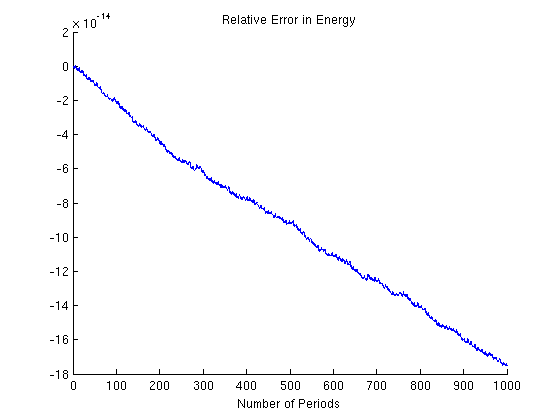
\includegraphics[width=0.75\textwidth]{error1.png}
    \label{test}
    \caption{Graphs of the conserved energy for the implicit midpoint scheme. The numerical solution was ran for 1000 wave periods. Spatial and temporal  discretisation were set to be 1 / 16. }
\end{figure}


\begin{figure}
    \centering
    \begin{subfigure}[b]{0.75\textwidth}
        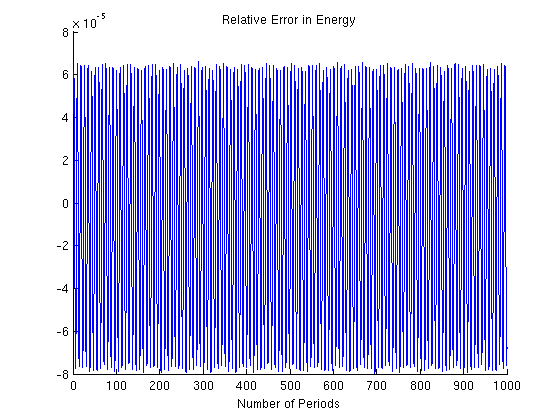
\includegraphics[width=\textwidth]{error2.png}
            \end{subfigure}
    ~ %add desired spacing between images, e. g. ~, \quad, \qquad, \hfill etc. 
      %(or a blank line to force the subfigure onto a new line)
    \begin{subfigure}[b]{0.75\textwidth}
        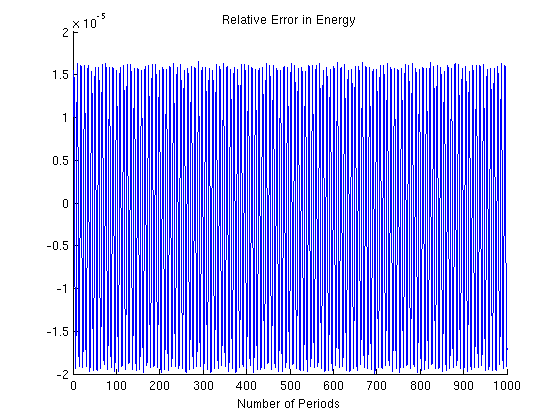
\includegraphics[width=\textwidth]{error3.png}
                \end{subfigure}
    ~ %add desired spacing between images, e. g. ~, \quad, \qquad, \hfill etc. 
    %(or a blank line to force the subfigure onto a new line)
  
    \caption{Graphs of the conserved shadow energy for the Stormer-Verlet scheme. The numerical solution was ran for 1000 wave periods. Spatial  discretisation was set to be 1 / 16. The above figure has a temporal discretisation 1/16 while the below figure has a temporal discretisation of 1/32. }\label{fig:animals}
      \label{test2}
\end{figure}

\subsection{ Error in density and velocity}

Tables \ref{midpointerror} and \ref{sverror} show the $L^2$ errors in velocity and density for both timestepper schemes. As expected the finite volume scheme is order 1 in space, such that the errors halved as we double the spatial resolution. The initial lack of convergence in the errors is due to not having enough elements to fully resolve the solution. it appears that 16-32 elements is enough to fully resolve the solution. It is worth noting that the energy conservation properties of these schemes was still preserved in small element systems, where the solution would be nonsensical due to growing errors in a long time scale.
What is surprising is that the implicit scheme was much faster than the explicit scheme in most of our timed runs, we believe that this is due to the simplicity of our problem such as being in one-dimensional space.  We then performed a stress test where we consider a scheme with 10, 000 elements to mimic a system with more variables or higher space dimensions. Table \ref{stresstest} collects the run times for the application of a single timestep to the system, as we expect the explicit system is much faster than the implicit scheme. 

% Please add the following required packages to your document preamble:
% \usepackage{booktabs}
\begin{table}[]
\centering
\caption{$L^2$ error and order of convergence of the numerical solution using an implicit midpoint timestepper after 10 wave periods. The timestep was taken to be equal to the spatial discretisation. We also present the run time of the solution to evaluate the efficiency of the two timesteppers. }
\label{midpointerror}
\begin{tabular}{@{}llllll@{}}
\toprule
     & \multicolumn{2}{l}{$\rho$} & \multicolumn{2}{l}{$u$}    & t (s)   \\ \midrule
   
$Nx$ & $L^2$ -error & Order       & $L^2$ -error & Order       &         \\
  \toprule
4    & 0.3062       &             & 1.1427       &             & 0.028   \\
8    & 0.5014       & 0.610690068 & 0.2472       & 4.622572816 & 0.03    \\
16   & 0.5263       & 0.952688581 & 1.2171       & 0.203105743 & 0.023   \\
32   & 1.1443       & 0.459931836 & 0.245        & 4.967755102 & 0.036   \\
64   & 0.6384       & 1.792449875 & 0.1895       & 1.292875989 & 0.054   \\
128  & 0.2954       & 2.161137441 & 0.1756       & 1.079157175 & 0.153   \\
256  & 0.1367       & 2.160936357 & 0.1063       & 1.651928504 & 0.443   \\
512  & 0.065        & 2.103076923 & 0.0574       & 1.851916376 & 2.338   \\
1024 & 0.0316       & 2.056962025 & 0.0297       & 1.932659933 & 21.055  \\
2048 & 0.0156       & 2.025641026 & 0.0151       & 1.966887417 & 173.044 \\ \bottomrule
\end{tabular}
\end{table}


% Please add the following required packages to your document preamble:
% \usepackage{booktabs}
\begin{table}[]
\centering
\caption{$L^2$ error and order of convergence of the numerical solution using a Stormer-Verlet timestepper after 10 wave periods. The timestep was taken to be equal to the spatial discretisation. We also present the run time of the solution to evaluate the efficiency of the two timesteppers.  }
\label{sverror}
\begin{tabular}{@{}llllll@{}}
\toprule
     & \multicolumn{2}{l}{$\rho$}               & \multicolumn{2}{l}{$u$}                  & t (s)  \\ \midrule
$Nx$ & L\textasciicircum 2 -error & Order       & L\textasciicircum 2 -error & Order       &        \\
 \toprule
4    & 0.2609                     &             & 1.1422                     &             & 0.029  \\
8    & 0.5057                     & 0.515918529 & 0.2468                     & 4.628038898 & 0.041  \\
16   & 0.5261                     & 0.961224102 & 1.2171                     & 0.202777093 & 0.03   \\
32   & 1.443                      & 0.364587665 & 0.245                      & 4.967755102 & 0.026  \\
64   & 0.6384                     & 2.260338346 & 0.1895                     & 1.292875989 & 0.043  \\
128  & 0.2954                     & 2.161137441 & 0.1756                     & 1.079157175 & 0.17   \\
256  & 0.1367                     & 2.160936357 & 0.1063                     & 1.651928504 & 0.775  \\
512  & 0.065                      & 2.103076923 & 0.0574                     & 1.851916376 & 4.371  \\
1024 & 0.0316                     & 2.056962025 & 0.0297                     & 1.932659933 & 52.62  \\
2048 & 0.0156                     & 2.025641026 & 0.0151                     & 1.966887417 & 535.08 \\ \bottomrule
\end{tabular}
\end{table}




% Please add the following required packages to your document preamble:
% \usepackage{booktabs}
\begin{table}[]
\centering
\caption{Run time for a numerical solution using 10, 000 elements. The solution was ran for a single timestep. }
\label{stresstest}
\begin{tabular}{@{}lll@{}}
      & Implicit Midpoint & Stormer-Verlet \\
$Nx$  & t (s)             & t(s)           \\
10000 & 255.226           & 0.788         
\end{tabular}
\end{table}




\end{document}